In Chapter~\ref{chp_preliminaries}, we have introduced the confined quasi-2D systems and the Ewald-splitting based summation methods.
In this chapter, we will focus on the Ewald2D summation and provide a comprehensive error analysis.
Then, we extend the Ewald2D summation to the case of dielectrically confined systems, i.e., the ICM-Ewald2D summation, and introduce its reformulation.
Finally, we provide a

\section{ICM-Ewald2D and its reformulation}\label{sec::icm_ewald2d}

For dielectric confined systems, combined with the ICM, the Ewald2D summation can be extended to accommodate for dielectric-confined systems.
In the ICM-Ewald2D summation~\cite{gan2024random}, Eqs.~\eqref{eq::Us_Ewald2D}-\eqref{eq::J0_Ewald2D} are modified as
\begin{equation}\label{eq::Uc}
    U_{s}^{\text{c}} =  \frac{1}{2} \sum_{i,j=1}^N \sum_{\bm{m}}{}^\prime \sum_{l=0}^M q_iq_{j \pm}^{(l)} \frac{\te{erfc}\left(\alpha \left|\bm{r}_i - \bm{r}_{j\pm}^{(l)}+ \V{\mathcal{M}}\right|\right)}{\left|\bm{r}_i-\bm{r}_{j\pm}^{(l)}+\V{\mathcal{M}}\right|}\;,
\end{equation}
\begin{equation}\label{eq::Fourier2D}
    U^{\te{c}}_{\ell} =  \frac{\pi}{2L_xL_y}\sum_{i, j=1}^N \sum_{l = 0}^{M} q_iq_{j \pm}^{(l)} \sum_{\V h\neq \V 0}\frac{e^{\i \V h\cdot \V r_{ij}}}{h}\mathcal{G}_{\alpha}(h,z_i - z_{j \pm}^{(l)})  - \frac{\alpha}{\sqrt{\pi}}\sum_{i=1}^{N}q_i^2+\mathcal{J}^{\te{c}}_0\;.
\end{equation}
Here $q_{j\pm}^{(l)}=\gamma_{\pm}^{(l)}q_j$ are the $l$-th layer image charge  strengths (with $l = 0$ terms indicating the original source charges), and the $\V 0$-th mode correction term should be modified accordingly as 
\begin{equation}\label{eq:ewald2d-j0}
    \mathcal J_0^c = -\frac{\pi}{L_xL_y}\sum_{i,j=1}^{N}\sum_{l=0}^{M} q_iq_{j\pm}^{(l)}\mathcal{G}_{\alpha}^0(|z_i-z_{j\pm}^{(l)}|)\;.
\end{equation}
Eqs.~\eqref{eq::Uc}--\eqref{eq:ewald2d-j0} integrate the well-established Ewald2D summation formula~\cite{parry1975electrostatic,zhonghanhu2014JCTC} for homogeneous systems with the ICM representation to account for polarization contributions. 
The resulting ICM-Ewald2D formula effectively performs a quasi-2D lattice summation on a system augmented in $z$ by a factor of $2M+1$. 
By selecting a sufficiently large $M$ and setting the real space and reciprocal space cutoffs as $r_c=s/\alpha$ and $k_c=2s\alpha$, respectively, where $s>0$ is a parameter, 
the error due to cutoffs has been estimated as $\sim O(e^{-s^2}/s^2)$~\cite{gan2024fast}, which decays rapidly as $s$ increases. 
However, the pairwise summation terms (over $i$ and $j$) in Eqs.~\eqref{eq::Fourier2D} and \eqref{eq:ewald2d-j0} still lead to a computational complexity of $O(N^2)$, requiring further acceleration techniques.
A widely used approach for acceleration is to reformulate the Ewald2D summation into a triply-periodic Ewald3D summation.
It is noteworthy that for homogeneous systems, such a reformulation was rigorously established by Pan and Hu~\cite{pan2014rigorous}. 
In what follows, we extend their approach to dielectric-confined systems.


First, one can rewrite the function~$\mathcal{G}_{\alpha}(h,z)$ in Eq.~\eqref{eq::G_Ewald2D} into an integral form:
\begin{equation}\label{eq::Ga-integral}
    \mathcal{G}_{\alpha}(h,z) = \int_{-\infty}^{\infty}\frac{e^{-\frac{h^2}{4\alpha^2}-t^2}}{\frac{h^2}{4\alpha^2}+t^2}e^{2\i \alpha z t} dt\;,
\end{equation}
and analogously,
\begin{equation}
\label{eq::J0-integral}
    \mathcal G_{\alpha}^{0}(z)=-\frac{1}{2\pi\alpha }\int_{-\infty}^{\infty}\frac{e^{-t^2}e^{2\i \alpha zt}-1}{t^2}dt\;.
\end{equation}
Discretizing the integrals in Eqs.~\eqref{eq::Ga-integral} and \eqref{eq::J0-integral} using the trapezoidal rule with mesh size $\pi/(\alpha L_z)$, where $L_z>H$ is a parameter, and substituting the discretized forms into Eq.~\eqref{eq::Fourier2D} gives
%By commutating the $i,j$-index of Eq.~\eqref{eq::J0-integral} and using the fact that $z_{ij}=-z_{ji}$, the first-order term on the numerator is eliminated and both of the integrands are smooth and exponentially decaying. Hence discretizing the integrals via trapezoidal rule yields spectral convergence~\cite{trefethen2014Rev}, which provides an approximation of Eq.~\eqref{eq::Uc} that
\begin{equation}\label{eq::UcFour}
\begin{split}
    U^{\T c}_{\ell} = \frac{2\pi}{L_xL_yL_z}\sum_{\bm{k}\neq \bm{0}}\frac{e^{-\frac{k^2}{4\alpha^2}}}{k^2}\rho_{\bm{k}}\bar{\rho}_{\bm{k}}^{M}-\frac{\alpha}{\sqrt{\pi}}\sum_{i=1}^{N}q_i^2+ U_{\T {YB}}^{M}+U_{\T {ELC}}^{M}+U_{\T{Trap}}^{M}\;,
\end{split}
\end{equation}
where $\bm{k}=2\pi(n_x/L_x,n_y/L_y,n_z/L_z)$ denotes the 3D periodic lattice vector, and the structure factors $\rho_{\bm{k}}$ and $\widetilde{\rho}_{\bm{k}}^{M}$ are defined as
\begin{equation}
    \rho_{\bm{k}} := \sum_{i=1}^{N}q_ie^{\i \bm{k}\cdot \bm{r}_i}\;,~
    \widetilde{\rho}_{\bm{k}}^{M} := \sum_{j=1}^{N}q_j\left[e^{-\i \bm{k}\cdot \bm{r}_i}+\sum_{l=1}^{M}\left(\gamma_{+}^{(l)}e^{-\i \bm{k}\cdot \bm{r}_{j+}^{(l)}}+\gamma_{-}^{(l)}e^{-\i \bm{k}\cdot \bm{r}_{j-}^{(l)}}\right)\right]\;.
\end{equation}
On the RHS of Eq.~\eqref{eq::UcFour}, the first two terms resemble the standard Ewald3D summation (with added \emph{vacuum layer} in $z$), where the second term accounts for the self-energy correction. 
The remaining terms provide the additional components required to correct Ewald3D back to Ewald2D:
\begin{equation}\label{eq:U^M_YB}
U_{\T {YB}}^{M}:=\frac{2\pi}{L_xL_yL_z}\left(\sum_{i=1}^{N}q_{i}z_{i}\right)\sum_{j=1}^{N}q_j\left[z_{j}+\sum_{l=1}^{M}\left(\gamma_{+}^{(l)}z_{j+}^{(l)}+\gamma_{-}^{(l)}z_{j-}^{(l)}\right)\right]\;,
\end{equation}
%and
\begin{equation}\label{eq:U^M_ELC}
U_{\T {ELC}}^{M}:=\frac{2\pi}{L_xL_y}\sum_{i,j=1}^{N}q_iq_j\sum_{\bm{h}\neq \bm{0}} \frac{e^{\i \bm{h}\cdot\bm{r}_{ij}}}{h}\frac{\cosh(hz_{ij})+\mathscr{F}_{\text{ELC}}^M(z_i,z_j)}{1-e^{hL_z}}\;,
\end{equation}
where $\mathscr{F}_{\text{ELC}}^M(z_i,z_j)$ is defined as:
\begin{equation}\label{eq::23}
\mathscr{F}_{\text{ELC}}^M(z_i,z_j):=\sum\limits_{l=1}^{M}\left[\gamma_{+}^{(l)}\cosh(h(z_i-z_{j+}^{(l)}))+\gamma_{-}^{(l)}\cosh(h(z_i-z_{j-}^{(l)}))\right].
\end{equation}
The terms in Eqs.~\eqref{eq:U^M_YB} and~\eqref{eq:U^M_ELC} correspond to the ICM-YB~\cite{yuan2021particle} and ICM-ELC~\cite{tyagi2008electrostatic} corrections, respectively. 
The remainder term, $U^{M}_{\T {trap}}$, emerges from the error introduced by trapezoidal discretization. 
The integrand in Eq.~\eqref{eq::Ga-integral} contains two simple poles at $t=\pm {\T i}h/(2\alpha)$, allowing for the estimation of discretization error using contour integral techniques~\cite{trefethen2014Rev}. 
Additionally, the integrand in Eq.~\eqref{eq::J0-integral} is smooth, %with its first-order term canceled due to the antisymmetry of $z_{ij}=-z_{ji}$ and the charge neutrality condition when substituted into Eq.~\eqref{eq::Fourier2D}, 
ensuring spectral convergence of the discretization. 
By applying an analysis analogous to that of Pan and Hu~\cite{pan2014rigorous}, we obtain $|U_{\text{trap}}^{M}|\sim e^{-\alpha^2(L_z-H)^2}$, which becomes negligible for $L_z \gg H$.  

Specially, for the case~$\gamma_{\T u}=\gamma_{\T d}=0$, i.e., the system is homogeneous, the long-range component is given by:
\begin{equation}\label{eq::U3D_Four}
	\begin{split}
		U_{\ell} = \frac{2\pi}{L_xL_yL_z}\sum_{\bm{k}\neq \bm{0}}\frac{e^{-\frac{k^2}{4\alpha^2}}}{k^2}\rho_{\bm{k}}\bar{\rho}_{\bm{k}} - \frac{\alpha}{\sqrt{\pi}}\sum_{i=1}^{N}q_i^2+ U_{\T {YB}} + U_{\T {ELC}} + U_{\T{Trap}}\;,
	\end{split}
\end{equation}
where $U_{\T {YB}}$ and $U_{\T {ELC}}$ are defined as:
\begin{equation}\label{eq::U3D_YB}
	U_{\T {YB}} := \frac{2\pi}{L_xL_yL_z}\left(\sum_{i=1}^{N}q_{i}z_{i}\right)\sum_{j=1}^{N}q_j z_{j}\;,
\end{equation}
%and
\begin{equation}\label{eq::U3D_ELC}
	U_{\T {ELC}} := \frac{2\pi}{L_xL_y}\sum_{i,j=1}^{N}q_iq_j\sum_{\bm{h}\neq \bm{0}} \frac{e^{\i \bm{h}\cdot\bm{r}_{ij}}}{h}\frac{\cosh(hz_{ij})}{1-e^{hL_z}}\;.
\end{equation}


In practical computations, the first term in Eq.~\eqref{eq::UcFour} can be efficiently calculated using fast algorithms such as the FFT~\cite{yuan2021particle}, the periodic FMM~\cite{pei2023fast}, and the random batch importance sampling~\cite{liang2022improved}, achieving computational complexities of $O(N\log N)$ or $O(N)$. 
Note that the ICM-YB correction term $U_{\T {YB}}^{M}$ can be directly computed with a cost of $O(N)$, and the remainder term $U_{\text{trap}}^M$ can be eliminated by appropriately choosing $L_z$.
% This parameter selection strategy is employed in the recently proposed ICM-Ewald3D~\cite{dos2015electrolytes} and ICM-PPPM~\cite{yuan2021particle} methods. 
% However, it is important to note that this approach overlooks the influence of the ICM-ELC correction term $U_{\T {ELC}}^{M}$, which may introduce significant errors. 
% Additionally, a rigorous estimate of the image truncation error is also absent in existing works. 
% In this study, we address and unify both sources of error.

\section{Accurate error estimates in Ewald summation for dielectrically confined Coulomb systems}

In this section, we present a comprehensive error analysis for both energy and force calculations, addressing the truncation error of the image charge series and the errors arising from the reformulation of the ICM-Ewald2D summation. 
We also perform extensive numerical experiments to validate our error analysis.
We will focus on force-related results in the main text, while energy-related findings are provided in Section~\ref{sec:numeric_energy}.
It is also important to note that in practical computations, the use of FFT can introduce additional errors due to particle spreading onto the uniform grid and the finite resolution of the grid. 
Since these error sources have been thoroughly analyzed in the literature~\cite{deserno1998mesh,wang2012numerical,liang2023error,wang2016multiple,barnett2019parallel,barnett2021aliasing} and are separable from the error discussed in this work, we refer interested readers to these works for more details.

\subsection{Truncation error of the image charge series}\label{sec:error_image}

In this subsection, we analyze the error introduced by truncating the infinite series of image charges at the $M$-th layer. 
This is achieved by reformulating the summation of the infinite image charge series as a Fourier expansion in the periodic $xy$ dimensions and as a geometric series in $z$. 

First, 
let $f(\bm r)$ be a smooth function for $\bm r\in\mathbb R^3$ which decays at infinity, with its Fourier transform denoted as $\widetilde{f}$, then we define the \emph{doubly-periodization} of $f$ as the following lattice sum:
\begin{equation}
f_{\mathcal M} (\bm r)=\sum_{\boldsymbol{m}\in\mathbb{Z}^2} f(\boldsymbol{r}+\V{L}_{\bm{m}})\;,
\end{equation}
and one has the following Poisson summation formula for $f_{\mathcal M} (\bm r)$:
\begin{equation}\label{eq:poissonsum}
f_{\mathcal M} (\bm r)=\frac{1}{2 \pi L_x L_y} \sum_{\bm{k}_{\bm{\rho}}} \int_{\mathbb{R}} \tilde{f}(\bm{k}_{\bm{\rho}}, k_z) e^{\i \bm{k}_{\bm{\rho}} \cdot \boldsymbol{\rho}} e^{\i k_z z} d k_z,
\end{equation}
where $\bm{r}=(\bm{\rho},z)$ with $\bm{\rho}:=(x,y)$, and $\bm{k}_{\bm{\rho}}=2\pi(n_x/L_x,n_y/L_y)$ with $n_x,n_y\in\mathbb{Z}$. 
Applying the Poisson summation formula Eq.~\eqref{eq:poissonsum} to Eq.~\eqref{eq:U_direct} yields 
\begin{equation}\label{eq::33}
    \begin{split}
        U = & \frac{1}{2}\sum_{i,j=1}^{N}q_iq_j\sum_{\bm{m}}{}^\prime\frac{1}{\left|\bm{r}_{ij}+\V{L}_{\bm{m}}\right|} \\
        & + \frac{\pi}{L_xL_y}\sum_{i,j=1}^{N}q_iq_j\sum_{\bm{h}\neq \bm{0}}\frac{e^{-\i \bm{h}\cdot\bm{r}_{ij}}}{h}  \sum\limits_{l=1}^{\infty}\left[\gamma_+^{(l)}e^{-h\left|z_i-z_{j+}^{(l)}\right|}+\gamma_-^{(l)}e^{-h\left|z_i-z_{j-}^{(l)}\right|}\right] \;,
    \end{split}
\end{equation}
where the first term represents the Coulomb energy of a homogeneous quasi-2D system and the second term accounts for the contribution from the image charges. Note that the contribution of the $\bm{h}=\bm{0}$ mode is contained in the homogeneous term, not relevant in the error analysis here for the image charge series.
Now if the image charge series is truncated at the $M$-th layer, then the discarded truncation error term is given by
\begin{equation}\label{eq:trucation_error}
U_{\text{err}}=\frac{\pi}{L_xL_y}\sum_{i,j=1}^{N}q_iq_j\sum_{\bm{h}\neq \bm{0}}\frac{e^{-\i \bm{h}\cdot\bm{r}_{ij}}}{h}\mathcal{G}_{M}(z_i,z_j)\;,  %
\end{equation}
where 
\begin{equation}\label{eq::rGrrij}
 \begin{split}
        \mathcal{G}_{M}(z_i,z_j)&:=\sum\limits_{l=M+1}^{\infty}\left[\gamma_+^{(l)}e^{-h\left|z_i-z_{j+}^{(l)}\right|}+\gamma_-^{(l)}e^{-h\left|z_i-z_{j-}^{(l)}\right|}\right]\; \\
        &= \sum\limits_{l = M + 1}^{\infty} \left[ \gamma_{\T u}^{\lfloor \frac{l}{2} \rfloor}\gamma_{\T d}^{\lceil \frac{l}{2} \rceil} e^{-h (2 \lceil \frac{l}{2} \rceil H + (-1)^l z_i - z_j)} + \gamma_{\T u}^{\lceil \frac{l}{2} \rceil}\gamma_{\T d}^{\lfloor \frac{l}{2} \rfloor} e^{-h (2 \lfloor \frac{l}{2} \rfloor H - (-1)^l z_i + z_j)} \right]\;.
    \end{split}
\end{equation}

To estimate $U_{\text{err}}$, we use the fact that $\mathcal{G}_{M}(z_i,z_j)$ can be reformulated as a geometric series. By inserting the definitions of $\gamma_{\pm}^{(l)}$ and $z_{j \pm}^{(l)}$ into Eq.~\eqref{eq::rGrrij}, we obtain 

\begin{equation}
    \begin{split}
        \mathcal{G}_{M}(z_i,z_j) = & \sum_{n = \frac{M + 1}{2}}^{\infty} \gamma_{\T u}^n \gamma_{\T d}^n e^{-2nhH} \left[ e^{- h z_{ij}} + e^{h z_{ij}} + \gamma_{\T u} e^{- h (z_i + z_j)} + \gamma_{\T d} e^{- h (2 H  - z_i - z_j)}\right] \\
        %= & (\gamma_{\T u} \gamma_{\T d})^{\frac{M + 1}{2}} e^{- (M +1) H h} \sum_{n = 0}^{\infty} \left( \gamma_{\T u} \gamma_{\T d} e^{- 2hH} \right)^n \left[ e^{-h z_{ij}} + e^{h z_{ij}} + \gamma_{\T d} e^{- h (2 H - z_i - z_j)} + \gamma_{\T u} e^{- h (z_i + z_j)} \right] \\
        = & (\gamma_{\T u} \gamma_{\T d})^{\frac{M + 1}{2}} e^{- (M +1) H h} \frac{\left[e^{-h z_{ij}} + e^{h z_{ij}} + \gamma_{\T u} e^{- h (z_i + z_j)} + \gamma_{\T d} e^{- h (2 H - z_i - z_j)} \right] }{1 - \gamma_{\T u} \gamma_{\T d} e^{-2hH}} \;,
    \end{split}
\end{equation}
for odd $M$, and 
\begin{equation}
    \begin{split}
        & \mathcal{G}_M(z_i,z_j) \\
        = & \sum_{n = \frac{M}{2}}^{\infty}  \gamma_{\T u}^n \gamma_{\T d}^n e^{- 2nhH} \left[  \gamma_{\T u} \gamma_{\T d} e^{- h (2 H  + z_{ij})} + \gamma_{\T u} \gamma_{\T d}  e^{- h (2 H  - z_{ij})} + \gamma_{\T u} e^{- h (z_i + z_j)} + \gamma_{\T d} e^{- h (2H  - z_i - z_j)} \right] \\
        = & (\gamma_{\T u} \gamma_{\T d})^{\frac{M}{2}} e^{- M H h} \frac{\left[ \gamma_{\T u} \gamma_{\T d} e^{- h (2 H + z_{ij})} + \gamma_{\T u} \gamma_{\T d} e^{- h (2H - z_{ij})} + \gamma_{\T u} e^{ - h (z_i + z_j)} + \gamma_{\T d} e^{-h (2 H - z_i - z_j)} \right]}{1 - \gamma_{\T u} \gamma_{\T d} e^{-2hH}}  \;,
    \end{split}
\end{equation}
for even $M$. In both cases, we obtain the following error bound:
\begin{equation}\label{eq:beta_ij}
    \abs{ \mathcal{G}_{M}(z_i,z_j) } \leq \abs{\gamma_{\T u} \gamma_{\T d} e^{- 2 H h}}^{\lfloor{(M+1)/2}\rfloor} \frac{\abs{\gamma_{\T u}} + \abs{\gamma_{\T d}} + 2 \abs{\gamma_{\T u} \gamma_{\T d}}}{1 - \abs{\gamma_{\T u} \gamma_{\T d}} e^{-2hH}} \leq \frac{4 \abs{\gamma_{\T u} \gamma_{\T d} e^{- 2 H h}}^{\lfloor{(M+1)/2}\rfloor}}{1 - \abs{\gamma_{\T u} \gamma_{\T d}} e^{-2hH}} \;,
\end{equation}
where we use the fact that 
\begin{equation}
    \begin{split}
        & ~ \abs{\gamma_{\T u} \gamma_{\T d}} e^{-h(2 H + z_{ij})} + \abs{\gamma_{\T u} \gamma_{\T d}} e^{ - h (2 H - z_{ij})} + \abs{\gamma_{\T d}} e^{- h (2 H - z_i - z_j)} + \abs{\gamma_{\T u}} e^{- h (z_i + z_j)} \\
        \leq & ~ 2 \abs{\gamma_{\T u} \gamma_{\T d}} +\abs{\gamma_{\T d}} + \abs{\gamma_{\T u}} \leq 4 \;.
    \end{split}
\end{equation}
Substituting Eq.~\eqref{eq:beta_ij} into Eq.~\eqref{eq:trucation_error}, we have

\begin{equation}\label{eq:U_gamma_bound}
    \begin{split}
        \left|U_{\text{err}}\right| & \leq \frac{4 \pi}{L_x L_y}  \sum_{\bm{h}\neq \bm{0}}  \frac{\abs{\gamma_{\T u} \gamma_{\T d} e^{- 2 hH}}^{\lfloor \frac{M + 1}{2} \rfloor}}{h(1 - \abs{\gamma_{\T u} \gamma_{\T d}} e^{- 2hH})}\abs{\sum_{i,j=1}^{N}q_i q_j e^{-\i \bm{h}\cdot\bm{r}_{ij}}} \\
        & \leq \frac{4\pi}{L_x L_y} \frac{C_{q} \abs{\gamma_{\T u} \gamma_{\T d}}^{\lfloor{(M+1)/2}\rfloor}}{1 - \abs{\gamma_{\T u} \gamma_{\T d}} e^{- 4\pi H / \max\{L_x,L_y\}}} \sum_{\bm{h}\neq \bm{0}} \frac{e^{- 2 \lfloor{(M+1)/2}\rfloor hH}}{h}\\
        & \leq \frac{4\pi}{L_x L_y} \frac{C_{q} \abs{\gamma_{\T u} \gamma_{\T d}}^{\lfloor{(M+1)/2}\rfloor}}{1 - \abs{\gamma_{\T u} \gamma_{\T d}} e^{- 4\pi H / \max\{L_x,L_y\}}} \int_{\frac{2\pi}{\max\{L_x,L_y\}}}^{\infty} 2\pi h \frac{e^{- 2 \lfloor{(M+1)/2}\rfloor hH}}{h} \, \mathrm{d}h \\
        & = \frac{8 \pi^2}{L_x L_y} \frac{C_{q} \abs{\gamma_{\T u} \gamma_{\T d}}^{\lfloor{(M+1)/2}\rfloor} e^{-\frac{4 \pi H \lfloor{(M+1)/2}\rfloor}{\max\{L_x,L_y\}}}}{1 - \abs{\gamma_{\T u} \gamma_{\T d}} e^{- 4\pi H / \max\{L_x,L_y\}}},
    \end{split}
\end{equation}
where $C_q$ is the bound of $|\sum_{i,j}q_iq_je^{-\i \bm{h}\cdot\bm{r}_{ij}}|$, which depends on the charge distribution of the system. 
A rough bound is $C_q\leq \sum_{i,j}|q_iq_j|\leq N^2q_{\text{max}}^2$, where $q_{\text{max}}=\max_{i}|q_i|$ denotes the maximum strength of a single point charge. 
This estimate can be further refined based on prior knowledge of the charge distribution. 
For example, under the Debye-H\"uckel (DH) approximation~\cite{levin2002electrostatic,gan2024fast}, the bound can be tightened to $C_q\leq CNq_{\max}^2$, where $C$ is a constant independent of $N$. 
Either way, we have the following rate of convergence for $|U_{\text{err}}|$ in terms of the truncation parameter $M$:
\begin{equation}\label{eq:Uerr}
|U_{\text{err}}|\sim O\left(\abs{\gamma_{\T u} \gamma_{\T d}}^{\lfloor\frac{M+1}{2}\rfloor} e^{-\frac{4 \pi H \lfloor (M + 1)/2\rfloor}{\max\{L_x,L_y\}}}\right)\;.
\end{equation}

Next, we analyze the truncation error of the force exerted on the $i$-th particle. Using the definition $\bm{F}^i_{\T{err}}=-\nabla_{\bm{r}_i} U_{\text{err}}$ and taking the derivative in each direction, we obtain:
\begin{equation}\label{eq::Ferr}
    \left|\bm{F}^i_{\T{err}}\right| = \left|\nabla_{\bm{r}_i} U_{\text{err}}\right|\leq  \abs{\frac{2\sqrt{3}\pi}{L_xL_y} q_i \sum_{j=1}^{N} q_j\sum_{\bm{h}\neq \bm{0}} e^{-\i \bm{h}\cdot\bm{r}_{ij}}\sum\limits_{l = M + 1}^{\infty}\mathcal{G}_{M}(z_i,z_j)}, 
\end{equation}
where we use the identity $\partial_{z_i}\sum_{ij}\mathcal{G}_M(z_{i},z_{j})=2h\sum_{ij}\mathcal{G}_{M}(z_i,z_j)$, and the factor $\sqrt{3}$ accounts for three dimensions of the force field $\bm F$.  
Substituting Eq.~\eqref{eq:beta_ij} into Eq.~\eqref{eq::Ferr}, we have 
\begin{equation}
\begin{split}
 |F^{i}_{\text{err}}| %& \leq \abs{\frac{2\sqrt{3}\pi}{L_xL_y} q_i \sum_{j=1}^{N} q_j\sum_{\bm{h}\neq \bm{0}} e^{-\i \bm{h}\cdot\bm{r}_{ij}}\sum\limits_{l = M + 1}^{\infty}\mathcal{G}_{M}(z_i,z_j)}\\
 & \leq \frac{8\sqrt{3}\pi}{L_xL_y}  \frac{C_{Q} \abs{\gamma_{\T u} \gamma_{\T d}}^{\lfloor{(M+1)/2}\rfloor}}{1 - \abs{\gamma_{\T u} \gamma_{\T d}} e^{- 4\pi H / \max\{L_x,L_y\}}} \sum_{\bm{h}\neq \bm{0}} e^{- 2 \lfloor{(M+1)/2}\rfloor hH}\\
 & \leq \frac{8\sqrt{3}\pi}{L_xL_y} \frac{ C_Q\abs{\gamma_{\T u} \gamma_{\T d}}^{\lfloor{(M+1)/2}\rfloor}}{1 - \abs{\gamma_{\T u} \gamma_{\T d}} e^{- 4\pi H / \max\{L_x,L_y\}}} \int_{\frac{2\pi}{\max\{L_x,L_y\}}}^{\infty} 2\pi h e^{- 2 \lfloor{(M+1)/2}\rfloor hH} \, \mathrm{d}h \\
& = \frac{16\sqrt{3} \pi^2}{L_xL_y} \frac{C_Q \abs{\gamma_{\T u} \gamma_{\T d}}^{\lfloor{(M+1)/2}\rfloor}}{1 - \abs{\gamma_{\T u} \gamma_{\T d}} e^{- 4\pi H / \max\{L_x,L_y\}}}  \frac{\left[1 + \frac{2\pi \lfloor{(M+1)/2}\rfloor H}{\max\{L_x,L_y\}}\right]}{4 \lfloor{(M+1)/2}\rfloor^2 H^2} e^{- \frac{4\pi \lfloor{(M+1)/2}\rfloor H}{\max\{L_x,L_y\}}}\;,
\end{split}
\end{equation}
where the second inequality is derived from the monotonicity of the exponential function, and $C_Q=|q_{i}\sum_{j=1}^{N}q_je^{-\i\bm{h}\cdot \bm{r}_{ij}}|\leq Nq_{\text{max}}^2$. 
If the DH theory is applied, the prefactor $C_Q$ can be further tightened to $C_Q\leq Cq_{\max}^2$, where $C$ is a constant independent of $N$. 
Similarly, considering the rate of convergence in terms of $M$, we have
\begin{equation}\label{eq::Ferr1}
|\bm{F}^i_{\text{err}}| \sim O\left(\lfloor (M+1)/2\rfloor^{-1}\abs{\gamma_{\T u} \gamma_{\T d}}^{\lfloor\frac{M+1}{2}\rfloor} e^{-\frac{4\pi H \lfloor(M+1)/2\rfloor}{\max\{L_x,L_y\}}}\right)\;.
\end{equation}
Comparing Eq.~\eqref{eq::Ferr1} and Eq.~\eqref{eq:Uerr},
we observed that the error in force converge slightly faster than that of the energy by a factor of $\lfloor (M+1)/2\rfloor^{-1}$. 

To validate our theoretical predictions, we employ the ICM-Ewald2D summation (i.e., Eqs.~\eqref{eq::Uc} and~\eqref{eq::Fourier2D}) to calculate the relative errors in force, $\mathcal{E}_r = \max\limits_{i=1,\ldots,N}\frac{\abs{\bm{F}^i_{\text{err}}}}{\abs{\bm{F}^i}}$, as a function of $M$, the number of truncated image layers.
Without loss of generality, we examine charge-asymmetric systems containing $13$ divalent cations and $26$ monovalent anions, randomly distributed within the simulation cell. 
In all calculations, the dimensions of the simulation cell along the periodic directions are fixed as $L_x = L_y = 10$, while the aspect ratio of the system is adjusted by varying the cell height $H$. 
Recall that the reflection factors for the upper and lower dielectric interfaces are denoted as $\gamma_{\T u}$ and $\gamma_{\T d}$, respectively. 
Finally, unless otherwise specified, we always set the Ewald splitting parameter $s=6$ to ensure that the errors due to Ewald decomposition remain negligible. 



The numerical results are presented in Fig.~\ref{fig:icm_error_force} (a) and (b), where we examine the convergence rate of $\mathcal{E}_r$ under different aspect ratios $L_x / H$ and reflection factors $\gamma=\gamma_{\T u}=\gamma_{\T d}$, respectively.
All results demonstrate that the force errors decay exponentially as $M$ increases. 
Additionally, we observe that the errors decay slower as the aspect ratio $L_x / H$ (Fig.~\ref{fig:icm_error_force} (a)) and the reflection factor $\gamma$ (Fig.~\ref{fig:icm_error_force} (b)) increases, both are consistent with our theoretical predictions in Eq.~\eqref{eq::Ferr1}. 
Furthermore, to quantitatively validate our theoretical findings, we also plot the theoretical decay rates predicted by Eq.~\eqref{eq::Ferr1} as dashed lines in Fig.~\ref{fig:icm_error_force}, showing excellent agreement with our numerical results.
The results for relative errors in energy are documented in Section~\ref{sec:numeric_energy}, where similar conclusions hold.  

%In \Cref{fig:icm_error_force} (a) and (b), we maintained fixed values for the reflection rate and the system height, respectively. 
%The results indicate that the energy error decreases exponentially with the number of reflection levels, denoted as~$M$, and the speed of decay depends on the reflection rate $\gamma$ and the system height $H$.
%The inset illustrates that the slope of the fitting line corresponds to the theoretical value $\lg(\gamma e^{-2\pi H / L_x})$, aligning with the theoretical prediction in Eq.~\eqref{eq:F_gamma_bound}.
%Additionally, the results on the energy error are presented in the Section 1 of supporting information.

\begin{figure}[htbp]
    \centering
    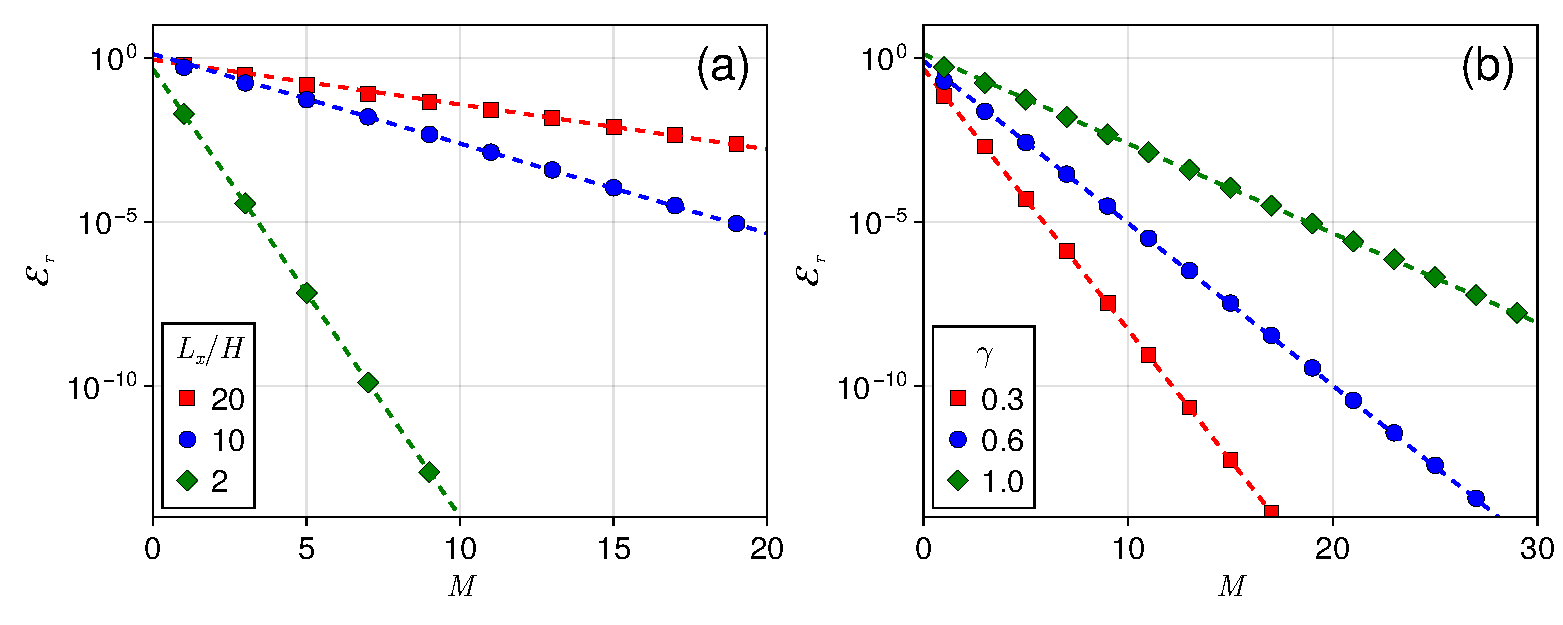
\includegraphics[width=0.98\linewidth]{figs/icm_error_force.pdf}
    \caption{
        Relative errors in force ($\mathcal{E}_r$) as a function of the truncation parameter $M$ for the image charge series. 
        The dashed lines represent the fitted curves with decay rates using our theoretical prediction Eq.~\eqref{eq::Ferr1}. 
        In panel (a), we fix $\gamma_{\T u} = \gamma_{\T d} = 1$ and consider systems with varying heights $H = 0.5$, $1$, and $5$. In panel (b), we fix $H = 1$ while varying $\gamma_{\T u} = \gamma_{\T d} = \gamma$ with values of $0.3, 0.6,$ and $1$. In both panels, we fix $L_x=L_y=10$.
    }
    \label{fig:icm_error_force}
\end{figure}

\subsection{Estimations of electrostatic layer correction (ELC) with image charges}\label{sec:error_reform}

Another often-overlooked source of error in existing algorithms stems from the omission of the ELC term in Eq.~\eqref{eq:U^M_ELC} and the discretization error using the trapezoidal rule, which has been discussed in Section~\ref{sec::icm_ewald2d}. 
In this section, we focus on deriving estimations of the ELC term with image charges.
%a rough estimation has been given as the following Lemma~\cite{gan2024fast}.

First, we recall the definition of the ELC term with image charges, denoted as $U_{\text{ELC}}^{M}$, as provided in the energy expressions Eqs.~\eqref{eq:U^M_ELC} and~\eqref{eq::23}:
\begin{equation}\label{eq::UELCm}
U_{\T {ELC}}^{M}:=\frac{2\pi}{L_xL_y}\sum_{i,j=1}^{N}q_iq_j\sum_{\bm{h}\neq \bm{0}} \frac{e^{\i \bm{h}\cdot\bm{r}_{ij}}e^{-hL_z}\left[\cosh(hz_{ij})+\mathscr{F}_{\text{ELC}}^{M}(z_i,z_j)\right]}{h(e^{-hL_z}-1)}\;.
\end{equation}
To derive an estimation for $U_{\T {ELC}}^{M}$, we introduce the following two inequalities. 
1). By basic algebraic manipulations, one obtains:  
\begin{equation}\label{eq::bpud1}
e^{-hL_z}\cosh(hz_{ij})\leq e^{-h(L_z-|z_{ij}|)}\leq e^{-h(L_z-H)}\;,
\end{equation}
and 2).
\begin{equation}\label{eq::bpud2}
\begin{split}
& e^{-hL_z}\mathscr{F}_{\text{ELC}}^{M}(z_i,z_j) \\
= & e^{-hL_z}\sum\limits_{l=1}^{M}\left[\gamma_{+}^{(l)}\cosh(h(z_i-z_{j+}^{(l)}))+\gamma_{-}^{(l)}\cosh(h(z_i-z_{j-}^{(l)}))\right]\\
= & \frac{1}{2}\sum\limits_{l=1}^{M}\left[\gamma_{+}^{(l)}e^{-h(L_z-|z_i-z_{j+}^{(l)}|)}+\gamma_{-}^{(l)}e^{-h(L_z-|z_i-z_{j-}^{(l)}|)}\right]+\frac{e^{-hL_z}}{2}(\mathcal{G}_{0}(z_i,z_j)-\mathcal{G}_{M}(z_i,z_j))\\
\leq & \frac{1}{2}\sum_{l=1}^{M}C^{(l)}_{\gamma}e^{-h(L_z-(l+1)H)}+\frac{(|\gamma_{\T u}|+|\gamma_{\T d}| + 2|\gamma_{\T u}\gamma_{\T d}|)e^{-hL_z}}{1-|\gamma_{\T u}\gamma_{\T d}|e^{-2hH}},
\end{split}
\end{equation}
where the factor $C^{(l)}_{\gamma}$ is defined as 
\begin{equation}
C^{(l)}_{\gamma}:=\left|\gamma_{+}^{(l)}\right|+\left|\gamma_{-}^{(l)}\right|=\left| \gamma_{\T d}^{\lceil l/2 \rceil} \gamma_{\T u}^{\lfloor l/2 \rfloor}\right|+\left| \gamma_{\T d}^{\lfloor l/2 \rfloor} \gamma_{\T u}^{\lceil l/2 \rceil}\right|.
\end{equation}
To obtain the above inequality, we use the definitions of $\gamma_{+}^{(l)}$ and $\gamma_{-}^{(l)}$, the bound $\max_{i,j}\{|z_i-z_{j+}^{(l)}|,|z_i-z_{j-}^{(l)}|\}\leq (l+1)H$, and the definition of $\mathcal{G}_{M}(z_i,z_j)$ in Eq.~\eqref{eq::rGrrij} along with its bound given in Eq.~\eqref{eq:beta_ij}. 
Substituting Eqs.~\eqref{eq::bpud1} and \eqref{eq::bpud2} into Eq.~\eqref{eq::UELCm} yields

\begin{equation}
\resizebox{.98\hsize}{!}{$
\begin{split}
\left|U_{\text{ELC}}^{M}\right|&\leq \frac{2\pi}{L_xL_y}\sum_{\bm{h}\neq \bm{0}} \frac{C_q\left[e^{-h(L_z-H)}+\frac{1}{2}\sum\limits_{l=1}^{M}C^{(l)}_{\gamma}e^{-h(L_z-(l+1)H)}+\frac{(|\gamma_{\T u}|+|\gamma_{\T d}| + 2|\gamma_{\T u}\gamma_{\T d}|)e^{-hL_z}}{1-|\gamma_{\T u}\gamma_{\T d}|e^{-\frac{4\pi H}{\max\{L_x,L_y\}}}}\right]}{h(1-e^{-\frac{2\pi L_z}{\max\{L_x,L_y\}}})}\\
&\leq \frac{4\pi^2 C_q}{L_xL_y(1-e^{-\frac{2\pi L_z}{\max\{L_x,L_y\}}})}\int^{\infty}_{\frac{2\pi}{\max\{L_x,L_y\}}} \left[e^{-h(L_z-H)}+\sum\limits_{l=1}^{M}\frac{C^{(l)}_{\gamma}}{2}e^{-h(L_z-(l+1)H)}+\frac{4e^{-hL_z}}{1-e^{-\frac{4\pi H}{\max\{L_x,L_y\}}}}\right]dh\\
&=\frac{4\pi^2 C_q}{L_xL_y(1-e^{-\frac{2\pi L_z}{\max\{L_x,L_y\}}})}\left[\frac{e^{-\frac{2\pi(L_z-H)}{\max\{L_x,L_y\}}}}{L_z-H}+\sum_{l=1}^{M}\frac{C_{\gamma}^{(l)}e^{-\frac{2\pi(L_z-(l+1)H)}{\max\{L_x,L_y\}}}}{2(L_z-(l+1)H)}+\frac{4e^{-\frac{2\pi L_z}{\max\{L_x,L_y\}}}}{L_z(1-e^{-\frac{4\pi H}{\max\{L_x,L_y\}}})} \right],
\end{split}
$}
\end{equation}
where we recall $C_q$ is the bound of $|\sum_{i,j=1}^{N}q_iq_je^{\i \bm{h}\cdot\bm{r}_{ij}}|$, $\left|\gamma_{\T u}\right|\leq 1$, and $\left|\gamma_{\T d}\right|\leq 1$. 
Finally, suppose $L_z>(M+1)H$, we obtain the following estimation for the ELC contribution in energy, $U_{\text{ELC}}^{M}$, as:
\begin{equation}
\label{eq::U_ELC}
\left|U_{\text{ELC}}^{M}\right|\sim O\left(e^{-\frac{2\pi(L_z-H)}{\max\{L_x,L_y\}}}+\sum_{l=1}^{M}C_{\gamma}^{(l)}e^{-\frac{2\pi(L_z-(l+1)H)}{\max\{L_x,L_y\}}}\right).
\end{equation}

The corresponding ELC term in force calculations can be estimated analogously. 
We have
\begin{equation}
\left|\bm{F}_{\text{ELC}}^{M,i}\right|:=|-\nabla_{\bm{r}_i} U_{\text{ELC}}^{M}|\leq \left|\frac{4\sqrt{3}\pi}{L_xL_y}q_i\sum_{j=1}^{N}q_j\sum_{\bm{h}\neq \bm{0}} \frac{e^{\i \bm{h}\cdot\bm{r}_{ij}}e^{-hL_z}\left[\cosh(hz_{ij})+\mathscr{F}_{\text{ELC}}^{M}(z_i,z_j)\right]}{1-e^{-hL_z}}\right|\;.
\end{equation}
Further applying the inequalities Eqs.~\eqref{eq::bpud1} and \eqref{eq::bpud2}, we obtain:

\begin{equation}
\resizebox{0.98\hsize}{!}{$
\begin{split}
\left|\bm{F}_{\text{ELC}}^{M,i}\right|\leq &\frac{4\sqrt{3}\pi}{L_xL_y}\sum_{\bm{h}\neq \bm{0}} \frac{C_Q\left[e^{-h(L_z-H)}+\frac{1}{2}\sum\limits_{l=1}^{M}C^{(l)}_{\gamma}e^{-h(L_z-(l+1)H)}+\frac{(|\gamma_{\T u}|+|\gamma_{\T d}| + 2|\gamma_{\T u}\gamma_{\T d}|)e^{-hL_z}}{1-|\gamma_{\T u}\gamma_{\T d}|e^{-\frac{4\pi H}{\max\{L_x,L_y\}}}}\right]}{1-e^{-\frac{2\pi L_z}{\max\{L_x,L_y\}}}}\\
\leq& \frac{8\sqrt{3}\pi^2 C_Q}{L_xL_y(1-e^{-\frac{2\pi L_z}{\max\{L_x,L_y\}}})}\int_{\frac{2\pi}{\max\{L_x,L_y\}}}^{\infty}h\left[e^{-h(L_z-H)}+\frac{1}{2}\sum\limits_{l=1}^{M}C^{(l)}_{\gamma}e^{-h(L_z-(l+1)H)}+\frac{4e^{-hL_z}}{1-e^{-\frac{4\pi H}{\max\{L_x,L_y\}}}}\right]dh\\
=&\frac{8\sqrt{3}\pi^2 C_Q}{L_xL_y(1-J_3)}\left[\frac{1+J_1}{(L_z-H)^2}e^{-J_1}+\sum_{l=1}^{M}\frac{C_{\gamma}^{(l)}(1+J_2^{(l)})}{2(L_z-(l+1)H)^2}e^{-J_2^{(l)}}+\frac{4(1+J_3)}{L_z^2(1-e^{-\frac{4\pi H}{\max\{L_x,L_y\}}})}e^{-J_3}\right]
\end{split}
$}
\end{equation}
where $C_Q$ is the bound of $|q_i\sum_{j=1}^{N}q_je^{-\i \bm{h}\cdot\bm{r}_{ij}}|$ and the coefficients $J_1$, $J_2^{(l)}$ and $J_3$ are defined via
\begin{equation}
J_1=\frac{2\pi(L_z-H)}{\max\{L_x,L_y\}},\quad\; J_2^{(l)}= \frac{2\pi(L_z-(l+1)H)}{\max\{L_x,L_y\}}\quad \;\text{and} \quad \; J_3=\frac{2\pi L_z}{\max\{L_x,L_y\}}.
\end{equation}
As before, by omitting all the prefactors, we arrive at the following estimation for the ELC contribution in force calculations:
\begin{equation}\label{eq::ForceError}
\left|\bm{F}_{\text{ELC}}^{M,i}\right|\sim O\left(e^{-\frac{2\pi(L_z-H)}{\max\{L_x,L_y\}}}+\sum_{l=1}^{M}C_{\gamma}^{(l)}e^{-\frac{2\pi(L_z-(l+1)H)}{\max\{L_x,L_y\}}}\right).
\end{equation}
Clearly, comparing Eq.~\eqref{eq::ForceError} and Eq.~\eqref{eq::U_ELC}, we find that the ELC contribution behaves asymptotically the same for both energy and force calculations.

\subsection{Leading-order analysis of the ELC term and numerical validations}\label{sec::leadingerr}
The theoretical estimations of the ELC term, as presented in Eqs.~\eqref{eq::ForceError} and~\eqref{eq::U_ELC}, behave differently under different system aspect ratios and reflection factors.
In this section, we conduct a detailed analysis of the leading-order contribution of the ELC term across different system parameter scenarios. 
Our focus will be on the analysis of force calculations, a similar approach can be applied to the energy.

First, by introducing two new dimensionless parameters $g_{\T u}:=\gamma_{\T u}e^{\frac{2\pi H}{\max\{L_x,L_y\}}}$ and $g_{\T d}:=\gamma_{\T d}e^{\frac{2\pi H}{\max\{L_x,L_y\}}}$, Eq.~\eqref{eq::ForceError} can be reformulated as
\begin{equation}
   \label{eq::Error_refo}
   \begin{aligned} \left|\bm{F}_{\text{ELC}}^{M,i}\right|&\sim e^{-\frac{2\pi(L_z-H)}{\max\{L_x,L_y\}}} \left[ 1 + \sum_{l=1}^{M} \left( g_{\T u}^{\lfloor \frac{l}{2} \rfloor} g_{\T d}^{\lceil \frac{l}{2} \rceil} + g_{\T u}^{\lceil \frac{l}{2} \rceil} g_{\T d}^{\lfloor \frac{l}{2} \rfloor} \right) \right]\\
   &=e^{-\frac{2\pi(L_z-H)}{\max\{L_x,L_y\}}}\left[(g_{\T u} + g_{\T d} + 2) \sum_{l = 0}^{\lfloor \frac{M - 1}{2} \rfloor} (g_{\T u}g_{\T d})^{l} + ((-1)^{M}+1) (g_{\T u}g_{\T d})^{\lfloor \frac{M}{2} \rfloor} - 1\right]\,.
   \end{aligned}
\end{equation}
From Eq.~\eqref{eq::Error_refo}, it is clear that the leading-order contribution of the ELC term depends on the magnitude of $|g_{\T u}g_{\T d}|$. 
Specifically, i). if $|g_{\T u}g_{\T d}| > 1$, the ELC leading-order term grows exponentially as $M$ increases:
\begin{equation}\label{eq::lhs_bigger1}
   \abs{\V{F}_{\text{ELC}}^{M,i}} =  \left\{
	\begin{aligned}
		& O \left(2 \abs{g_{\T u} g_{\T d}}^{M/2} e^{-\frac{2\pi (L_z - H)}{\max\{L_x,L_y\}}} \right) , & \text{if $M$ is even,}\\
		& O \left( \left(g_{\T u} + g_{\T d}+2\right)\abs{g_{\T u} g_{\T d}}^{\frac{M-1}{2}} e^{-\frac{2\pi (L_z -H)}{\max\{L_x,L_y\}}} \right) , & \text{if $M$ is odd.}
	\end{aligned}
	\right.
\end{equation} 
ii). If $|g_{\T u}g_{\T d}|=1$, the ELC leading-order term grows linearly with $M$:
\begin{equation}
\label{eq::lhs_1}
\abs{\V{F}_{\text{ELC}}^{M,i}} = O \left( \frac{M}{2}\left(g_{\T u} + g_{\T d}+2\right)e^{-\frac{2\pi L_z}{\max\{L_x,L_y\}}} \right)\;.
\end{equation}
iii). If $|g_{\T u}g_{\T d}|<1$, the summation in Eq.~\eqref{eq::Error_refo} converges as $M\rightarrow +\infty$, yielding a uniform estimation independent with $M$:
\begin{equation}
\label{eq::lhs_less1}
\abs{\V{F}_{\text{ELC}}^{M,i}} \sim O \left( \left(g_{\T u}+g_{\T d}+2\right)e^{-\frac{2\pi L_z}{\max\{L_x,L_y\}}} \right).
\end{equation}
The preceding analysis indicates that, for a fixed system size \( L_z \) (including vacuum layers), the numerical error associated with neglecting the ELC term exhibits a non-trivial dependence on the number of image charge layers \( M \). 
Specifically, for \( |g_{\T u}g_{\T d}|>1 \), the error grows exponentially with \( M \);
for \( |g_{\T u}g_{\T d}| = 1 \), it grows linearly; and for \( |g_{\T u}g_{\T d}| < 1 \), no error escalation is observed as \( M \) increases.

In what follows, we perform a series of numerical tests to validate our theoretical analysis. 
First, we examine the simplest case, i.e., systems \emph{without} dielectric interfaces by setting $\gamma_{\T u} = \gamma_{\T d} = 0$. 
In our numerical tests, we fix $L_x = L_y = 10$, and vary the system heights by setting $H = 0.5, 1, 5$. 
For clarity, we further introduce the dimensionless \emph{padding ratio} $R$, defined as $P = (L_z - H) / L_x$. 
The results, presented in Fig.~\ref{fig:elc_error_force}, clearly show that the relative errors in force $\mathcal{E}_r$ decay exponentially with $P$. 
Notably, the convergence with respect to $P$ is independent of the specific choice of $H$, aligning with our theoretical predictions in Eq.~\eqref{eq::ForceError}. 
Furthermore, our findings underscore the computational challenges of simulating \emph{strongly-confined} systems, characterized by a high aspect ratio, i.e., $L_x / H$. 
According to Fig.~\ref{fig:elc_error_force}, achieving single- or double-precision relative accuracy requires padding the system in the $z$ direction such that $(L_z - H)/L_x$ reaches around 3 and 5, respectively. For strongly-confined systems, this requires one to set $L_z\gg H$, which can significantly increases the computational cost if grid-based algorithms are used.

\begin{figure}[htbp]
    \centering
    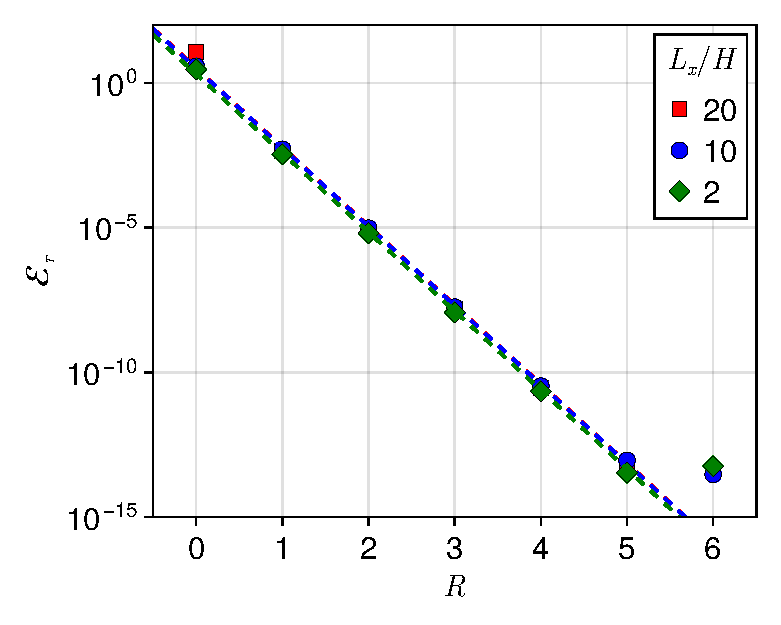
\includegraphics[width=0.55\linewidth]{figs/elc_error_force.pdf}
    \caption{Relative errors in force ($\mathcal{E}_r$) as a function of the padding ratio $R$ for systems without dielectric interfaces. 
    We consider systems with heights $H = 0.5, 1, 5$ while fixing $L_x=L_y=10$. The padding ratio is defined as $R = (L_z - H) / L_x$. The dashed lines represent the fitted curves with decay rates using theoretical prediction Eq.~\eqref{eq::ForceError}. }
    \label{fig:elc_error_force}
\end{figure}

Next, we examine systems with dielectric interfaces.
We set $\gamma_{\T u}=\gamma_{\T d}=\gamma$ and explore two prototypical scenarios by choosing $\gamma = 0.6$ and $1$, respectively. 
In both scenarios, the size of simulation box is fixed as $L_x=L_y=10$ and $H = 0.5$, and we vary the padding ratio $R$ (by changing $L_z$) and the image series truncation parameter $M$ to validate our theoretical results.
We first address the scenario with $\gamma = 0.6$, where we have $|g_{\T u}g_{\T d}| < 1$, so that the numerical errors are mainly contributed by the image series truncation error Eq.~\eqref{eq::Ferr1} and the ELC term Eq.~\eqref{eq::lhs_less1}.
% \begin{equation}\label{eq::0.6}
%     |\bm{F}_{\text{err}}^{M,i}| \sim \max \left\{ \lfloor(M+1)/2\rfloor^{-1}\left|\gamma_{\T u}\gamma_{\T d}\right|^{\lfloor\frac{M+1}{2}\rfloor} e^{-\frac{4\pi H\lfloor (M+1)/2\rfloor}{\max\{L_x,L_y\}}}, ~(g_{\T u}+g_{\T d}+2)e^{-\frac{2\pi L_z}{\max\{L_x,L_y\}}} \right\}\;.
% \end{equation}
The numerical results, as shown in Fig.~\ref{fig:error_icm_pad_gamma_0.6_force}, demonstrate that the errors in force decay exponentially with both the padding ratio $R$ and the number of image charge layers $M$, consistent with our theoretical predictions. Notice that in Fig.~\ref{fig:error_icm_pad_gamma_0.6_force} (a), the errors saturate at certain accuracy levels, this is due to the fixed image series truncation error (as we fix $M$). Similarly, the errors saturate in Fig.~\ref{fig:error_icm_pad_gamma_0.6_force} (b) as they reach the fixed ELC errors for given padding ratios $R$.
\begin{figure}[htbp]
    \centering
    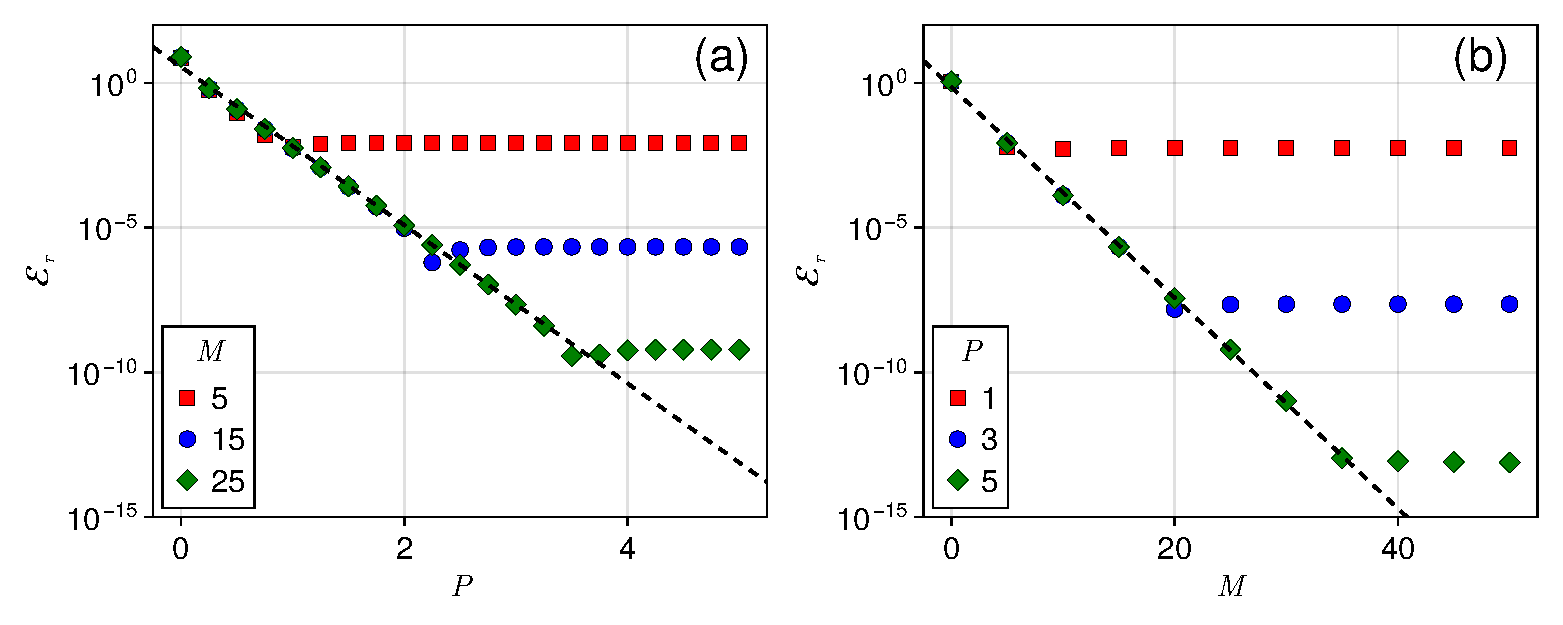
\includegraphics[width=0.98\linewidth]{figs/error_icm_pad_gamma_0.6_force.pdf}
    \caption{Relative errors in force ($\mathcal{E}_r$) for systems with dielectric interfaces. Here we fix $\gamma_{\T u}=\gamma_{\T d}=\gamma = 0.6$, $L_x=L_y=10$ and $H = 0.5$. 
    Panel (a) illustrates errors as a function of padding ratio $R$ with fixed image charge layers ($M=5,~15,~25$); panel (b) illustrates errors as a function of $M$ with fixed padding ratios ($R = 1,~3,~5$). The dashed lines in (a) and (b) represent the fitted curves with decay rates using theoretical predictions Eq.~\eqref{eq::lhs_less1} and Eq.~\eqref{eq::Ferr1}, respectively.}
    \label{fig:error_icm_pad_gamma_0.6_force}
\end{figure}

Now consider the scenario with $\gamma = 1$, where we have $|g_{\T u}g_{\T d}| > 1$, so that the numerical errors associated with the ELC term are described by Eq.~\eqref{eq::lhs_bigger1}.
In this context, the error behavior becomes more complex: as $M$ increases, the ELC error exhibits exponential growth, whereas the image truncation error decreases exponentially.
As illustrated in Fig.~\ref{fig:error_icm_pad_gamma_1_force} (a), by fixing $M$, we still observe exponential convergence in forces as the padding ratio $R$ increases. 
However, for a fixed padding ratio $R$, the errors display non-monotonic behavior with increasing $M$, as depicted in Fig.~\ref{fig:error_icm_pad_gamma_1_force} (b).
This subtle phenomenon was not fully understood since its first observation in the work of Yuan \emph{et al.}~\cite{yuan2021particle}. 
Our analysis reveals it as the combined effect of image truncation and ELC errors: 
initially, errors decrease due to the decay of image truncation errors; and once $M$ surpasses a certain $P$-dependent threshold, the error amplification mechanism predicted by Eq.~\eqref{eq::lhs_bigger1} becomes dominant, causing errors to grow exponentially.
Finally, we note that in strongly-confined systems, the presence of dielectric interfaces would introduce additional computational challenges~\cite{dos2015electrolytes}. 
Specifically, for systems with higher aspect ratios, a larger $M$ is required to achieve the same level of accuracy. The relevant numerical results are summarized in Section 2 of the SI. 
\begin{figure}[htbp]
    \centering
    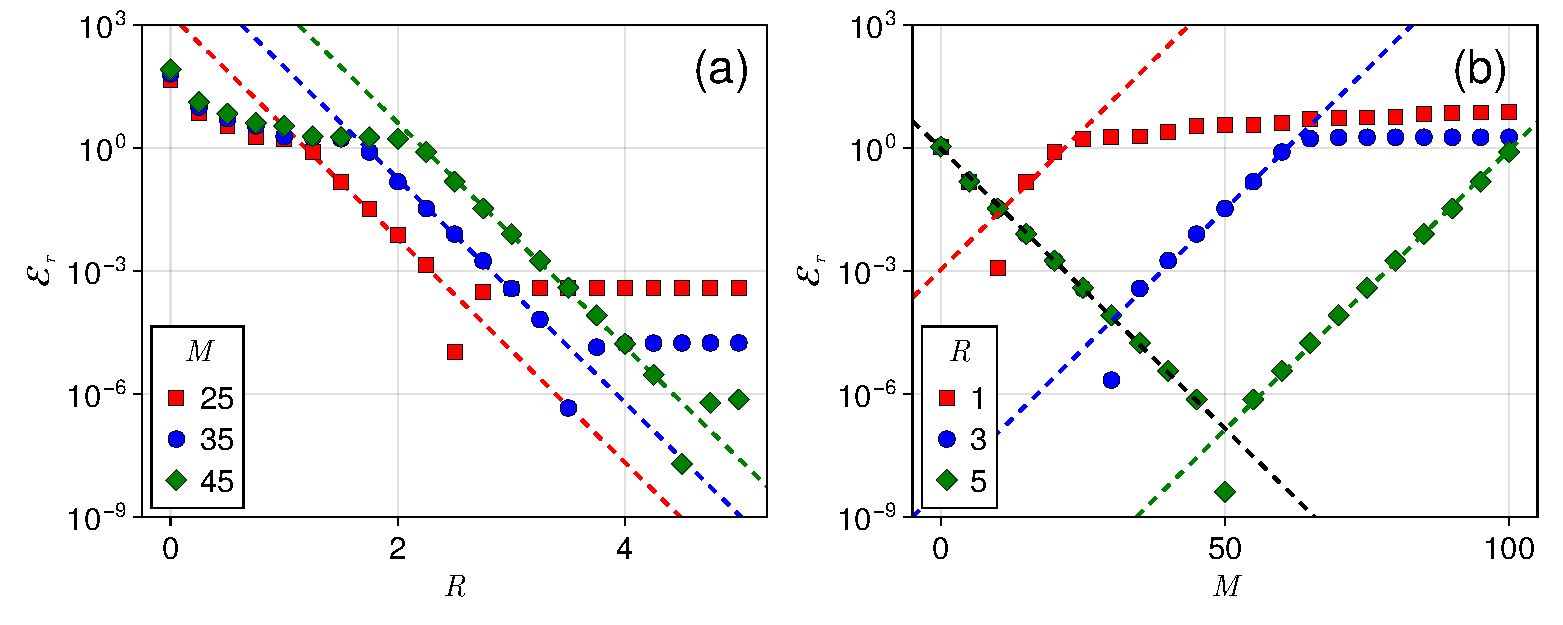
\includegraphics[width=0.98\linewidth]{figs/error_icm_pad_gamma_1_force.pdf}
    \caption{Relative errors in force ($\mathcal{E}_r$) for systems with dielectric interfaces. Here we fix $\gamma_{\T u}=\gamma_{\T d}=\gamma = 1$, $L_x=L_y=10$ and $H = 0.5$. 
    Panel (a) illustrates errors as a function of padding ratio $R$ with fixed image charge layers ($M=25,~35,~45$); panel (b) illustrates errors as a function of $M$ with fixed padding ratios ($R = 1,~3,~5$). The dashed lines in (a) and (b) represent the fitted curves with decay/growth rates using theoretical predictions Eq.~\eqref{eq::lhs_bigger1} and Eq.~\eqref{eq::Ferr1}.}
    \label{fig:error_icm_pad_gamma_1_force}
\end{figure}

% In practical simulations, especially when studying thin membranes, carbon nanotubes, and supercapacitors, accurately capturing the effects of nanoconfinement, i.e., when $H \ll \max\{L_x,L_y\}$, is crucial. Previous works have numerically shown that more image layers are needed to achieve satisfactory accuracy~\cite{dos2015electrolytes}. To further investigate the behavior of strongly confined systems, we present the error in force in \Cref{fig:icm_elc_error_force}, where we set $L_x=L_y=10$, $(L_z-H)/L_x = 5$ and consider system heights $H = 0.5, 1, 5$ while varying the number of image charge layers $M$. In \Cref{fig:icm_elc_error_force} (a), for $\gamma = 0.6$, we observe that the error decays exponentially as $M$ increases for $H = 0.5$ and $H = 1$. However, for $H = 5$, where $\gamma e^{2\pi H / L_x} > 1$, the error initially decreases before increasing as $M$ rises. This behavior is consistent with our theoretical predictions in Eqs.~\eqref{eq::FerrM} and \eqref{eq::FerrModd}. In \Cref{fig:icm_elc_error_force} (b), with $\gamma = 1$, we observe a similar pattern, where the error first decreases and then increases with increasing $M$. Furthermore, we note that the rate of increase depends on the aspect ratio $H/L_x$. A higher aspect ratio leads to a faster increase or decrease in error as $M$ is less or greater than the critical value that minimizes the error, respectively. This is also in alignment with our theoretical results in Eqs.~\eqref{eq::FerrM} and \eqref{eq::FerrModd}.

% \begin{figure}[htbp]
%     \centering
%     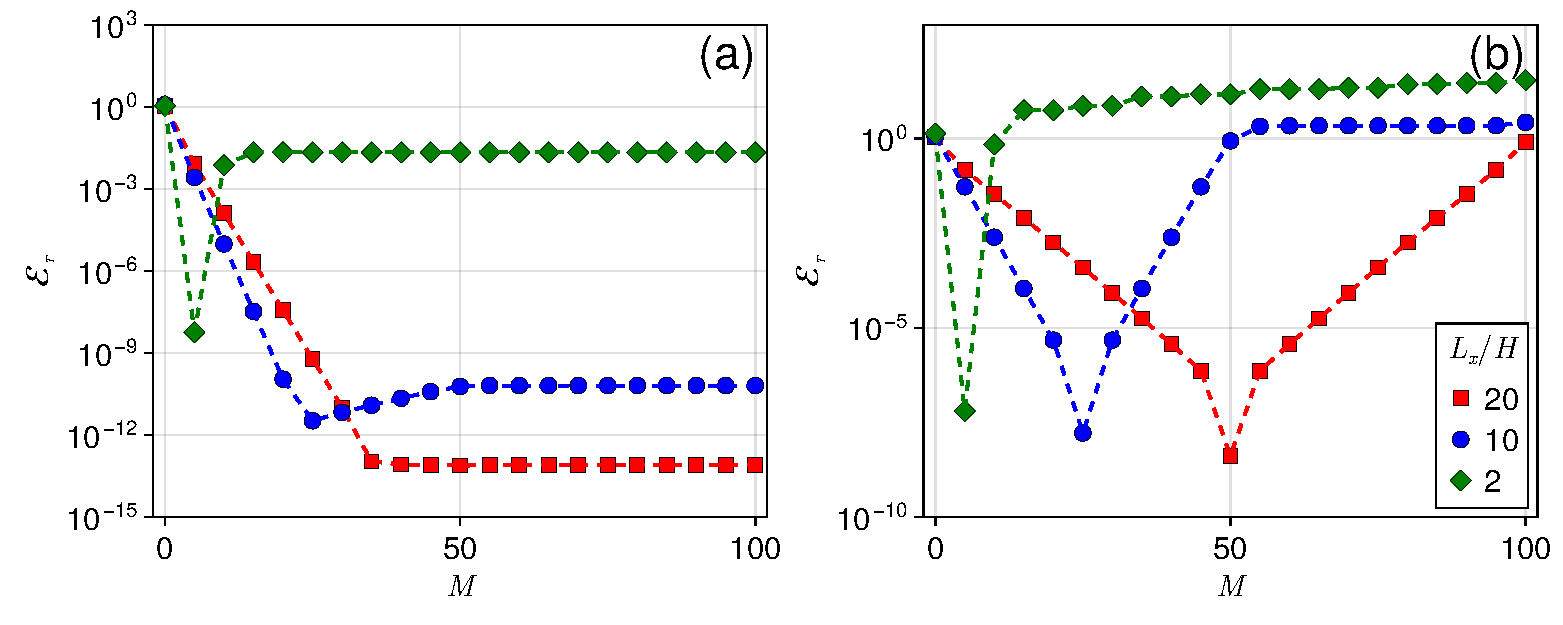
\includegraphics[width=0.98\linewidth]{figs/icm_elc_error_force.pdf}
%     \caption{Relative error of force ($\mathcal{E}_r$) in a dielectric-confined Coulomb system with parameters $P = 5$ and $H = 0.5, 1, 5$. In panels (a) and (b), the dielectric contrasts are set to $\gamma_{\T u} = \gamma_{\T d} = \gamma = 0.6$ and $\gamma_{\T u} = \gamma_{\T d} = \gamma = 1$, respectively.}
%     \label{fig:icm_elc_error_force}
% \end{figure}

As a final example, we validate our theoretical findings by replicating the non-monotonic error behavior reported by Yuan \emph{et al.} in figure 2 of Ref~\cite{yuan2021particle}. 
The reproduced numerical results are shown in Fig.~\ref{fig:error_yuan}, where we examine systems of dielectric-confined 2:1 electrolytes with $L_x = L_y = 15$ and $H = 5$. 
The three panels in Fig.~\ref{fig:error_yuan} correspond to systems with different reflection factors: $\gamma_{\T u} = \gamma_{\T d} = \gamma = 0.6$, $0.95$, and $1$, respectively. 
Within each panel, $L_z$ is varied as $45$, $75$, and $105$.
Note that for all cases considered here, the condition $|g_{\T u}g_{\T d}| > 1$ is satisfied, suggesting a similar phenomenon to that shown in Fig.~\ref{fig:error_icm_pad_gamma_1_force} (b), where errors diverge exponentially as $M$ surpasses a certain threshold.
Finally, we fit the numerical results using an analytical expression that combines the two primary error terms, Eq.~\eqref{eq:Uerr} and Eq.~\eqref{eq::U_ELC}, with coefficients determined through fitting.
The fitted curves, represented by dashed lines in Fig.~\ref{fig:error_yuan}, exhibit excellent agreement with the numerical data, thereby validating our theoretical predictions.

\begin{figure}[htbp]
\centering
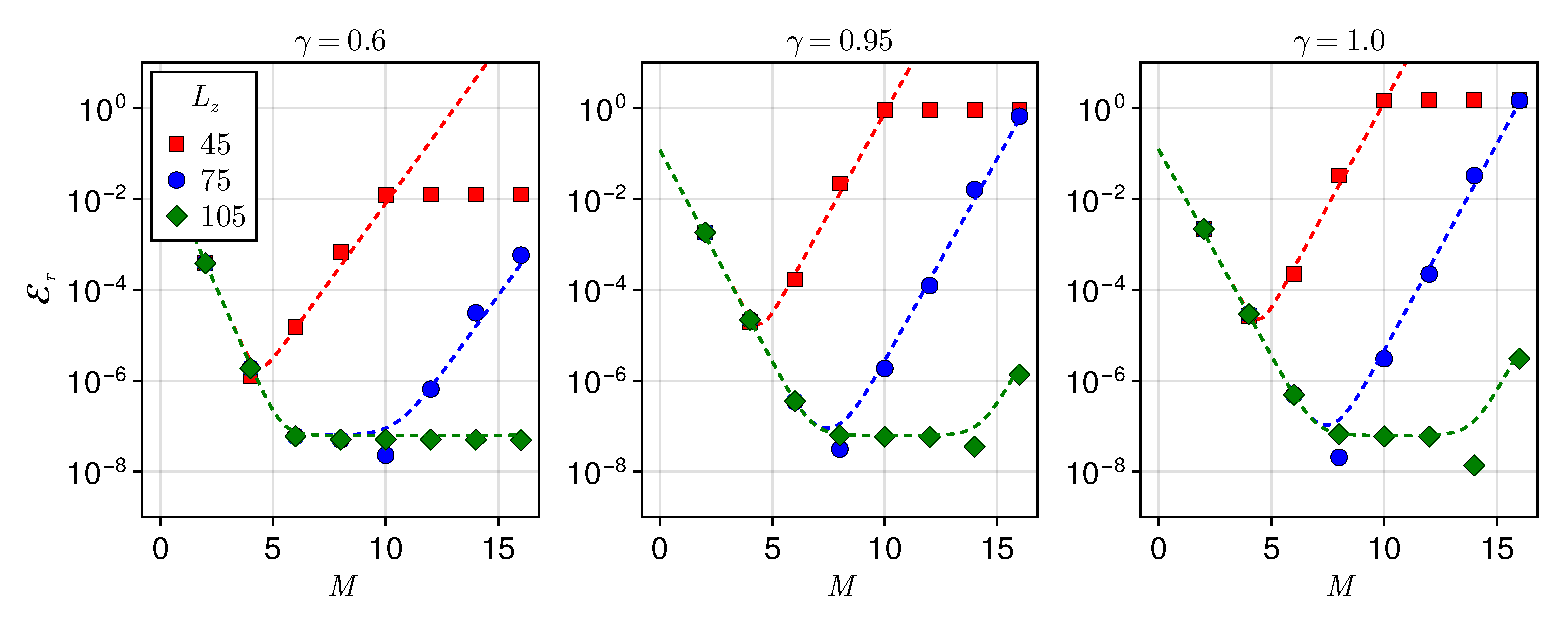
\includegraphics[width=0.98\linewidth]{figs/error_yuan.pdf}
\caption{
Relative errors ($\mathcal{E}_r$) in electrostatic energy for systems of 2:1 electrolytes with dieletric interfaces. 
Here we consider the same system setup studied by Yuan \emph{et al.}~\cite{yuan2021particle} using the ICM-PPPM method with $\gamma_{\T u}=\gamma_{\T d}=\gamma$ = 0.6, 0.95, and 1 (from left to right), respectively. In each panel, we fix $L_x = L_y = 15$, $H = 5$, and consider $L_z=$$45$, $75$, and $105$. 
Finally, the dashed lines represent the fitted curves using the sum of Eqs.~\eqref{eq:Uerr} and~\eqref{eq::U_ELC} (with coefficients determined by fitting).
}
\label{fig:error_yuan}
\end{figure}

\subsection{Optimal parameter selection strategy}\label{sec:parameter}
In practical simulations of dielectric-confined systems, a systematic strategy for determining the optimal algorithm parameters is highly beneficial. Specifically, given a prescribed error tolerance $\varepsilon$, it is crucial to identify parameter choices that achieve this tolerance with minimum computational cost. 
For ICM-Ewald3D~\cite{dos2015electrolytes} and ICM-PPPM~\cite{yuan2021particle} algorithms, 
our error analysis indicates that four interrelated parameters must be determined to control accuracy: 1). the Ewald splitting parameter $\alpha$, 2). the real-space cutoff $r_c$, 3). the image charge series truncation parameter $M$, and 4). the padding length $L_z$. 
By combining the error estimates from this study with the established Ewald splitting error, the overall error estimates for the ICM-Ewald3D and ICM-PPPM methods can be expressed as follows:
\begin{equation}\label{eq:error_icmelc}
\resizebox{0.8\width}{!}{\(
%|U_{\T{err}}|\sim|\bm{F}_{\T{err}}^{i}| 
\varepsilon \sim O\left(\frac{e^{-s^2}}{s^2}+\abs{\gamma_{\T u} \gamma_{\T d}}^{\lfloor\frac{M+1}{2}\rfloor} e^{-\frac{4\pi H \lfloor\frac{(M+1)}{2}\rfloor}{\max\{L_x,L_y\}}} + e^{-\frac{2\pi(L_z-H)}{\max\{L_x,L_y\}}} + \sum\limits_{l=1}^{M}C_{\gamma}^{(l)}e^{-\frac{2\pi(L_z-(l+1)H)}{\max\{L_x,L_y\}}}+e^{-\alpha^2 (L_z-H)^2}\right)\;,
\)}
\end{equation}
where the first term represents the Ewald decomposition error, the second term denotes the image charge series truncation error, the third and fourth terms correspond to the errors associated with the ELC term with image charges, and the last term corresponds to the trapezoidal discretization error.
Recall that, based on our analysis, the fourth term can grow exponentially with increasing $M$ if the condition $|g_{\T u}g_{\T d}| > 1$ is met. 
As a result, one should be careful in properly selecting the parameter $M$. 
Choosing a very large $M$ will not only increase the computational cost, but may also lead to incorrect results under certain circumstances.
In what follows, we propose an optimal parameter selection strategy based on the theoretical guidance of Eq.~\eqref{eq:error_icmelc}.

\emph{Step 1}: select $M$, so that the second term in Eq.~\eqref{eq:error_icmelc} is controlled by $\varepsilon$. 
There are three possible cases depending on the system setups:
\begin{enumerate}
    \item \textbf{Case 1}: If there is no dielectric interface, i.e., $\gamma_{\T u}=\gamma_{\T d}=0$, one simply set $M=0$.
    \item \textbf{Case 2}: If there is only one dielectric interface, i.e., either $\gamma_{\T u}=0$,$~\gamma_{\T d}\neq 0$ or $\gamma_{\T u}\neq 0$,$~\gamma_{\T d}=0$, one can set $M=1$ (since there is no image charge reflection).
    \item \textbf{Case 3}: If there are two polarizable dielectric interfaces, i.e., $\gamma_{\T u}\gamma_{\T d}\neq 0$, we select $M$ according to the following condition (obtained by algebraic manipulations of Eq.~\eqref{eq:Uerr}):
    \begin{equation}\label{eq::38}
    M\sim \frac{2\log \varepsilon - \frac{4\pi H}{\max\{L_x,L_y\}} - \log|\gamma_{\T u} \gamma_{\T d}|}{\log|\gamma_{\T u} \gamma_{\T d}| - \frac{4\pi H}{\max\{L_x,L_y\}}}\;.
\end{equation}
\end{enumerate}

\emph{Step 2}: select $L_z$, such that the sum of the third and fourth terms in Eq.~\eqref{eq:error_icmelc} is controlled by $\varepsilon$. 
Based on the leading-order error analysis presented in Section~\ref{sec::leadingerr}, two cases should be considered: 
\begin{enumerate}
    \item \textbf{Case 1}: If the condition $|g_{\T u}g_{\T d}|=\left|\gamma_{\T u}\gamma_{\T d}e^{\frac{4\pi H}{\max\{L_x,L_y\}}}\right|<1$
is satisfied, we have
\begin{equation}\label{eq::Lz_gamma_u_gamma_d_less1}
    L_z \geq H + \frac{\max\{L_x,L_y\}}{2\pi} \left( \log\frac{1}{\varepsilon} + \log \abs{\gamma_{\T u} + \gamma_{\T d} + e^{- \frac{2\pi H}{\max\{L_x,L_y\}}}} \right)\;.
\end{equation}
Note that for this case, $L_z$ can be chosen independent of $M$.
\item \textbf{Case 2}: If $\left|\gamma_{\T u}\gamma_{\T d}e^{\frac{4\pi H}{\max\{L_x,L_y\}}}\right|\geq 1$, we obtain
\begin{equation}\label{eq::Lz_gamma_u_gamma_d_greater1}
    L_z \geq (M + 1) H + \frac{\max\{L_x,L_y\}}{2\pi} \left( \log\frac{1}{\varepsilon} + \log \abs{\gamma_{\T u} \gamma_{\T d}} \right)\;.
\end{equation}
\end{enumerate}
It is interesting to note that, the selection of $L_z$ as derived in Eq.~\eqref{eq::Lz_gamma_u_gamma_d_greater1} can be interpreted physically as ensuring a sufficiently large vacuum layer in $z$ such that all the image charges can not overlap each other due to the periodic boundary conditions (necessitating $L_z\geq (M+1)H$). Additionally, an extra buffer zone is required, the length of which is determined by the specific tolerance $\varepsilon$.

\emph{Step 3}. After $M$ and $L_z$ are determined, the Ewald splitting parameter $\alpha$ and real-space cutoff $r_c$ can be selected. 
As indicated by Eq.~\eqref{eq:error_icmelc}, the Ewald decomposition error is independent of both the image truncation and the ELC error terms. 
The only extra constraint comes from the trapezoidal discretization error, which is typically minor due to its rapid decay with increasing $L_z$.
Consequently, the standard strategy can be employed to choose these parameters by setting $\varepsilon = e^{-s^2}/s^2$ and solving for $s$, where $s=r_c/\alpha$. 
The specific values of $r_c$ and $\alpha$ can then be adjusted to balance the computational costs between real-space and reciprocal-space calculations~\cite{frenkel2023understanding}.
Finally, to guarantee that the trapezoidal discretization error has been controlled, it is necessary to verify that the following condition is satisfied: 
\begin{equation}
    \alpha \geq (L_z-H)^{-1}\sqrt{\log\varepsilon^{-1}}\;.
\end{equation}
If this condition is not met, then $\alpha$ must be relaxed to fulfill this constraint.

We finally validate the proposed parameter selection strategy through numerical tests on two prototypical dielectric-confined systems, characterized by $\gamma_{\T u} = \gamma_{\T d} = 0.6$ and 1, respectively. 
The system dimensions are fixed at $L_x=L_y=10$ and $H = 1$. 
Note that for the system with $\gamma=0.6$, we have $|g_{\T u}g_{\T d}|<1$, while for the system with $\gamma=1$, $|g_{\T u}g_{\T d}|>1$.
For each system, the error tolerance $\varepsilon$ is set to $\epsilon = 10^{-4}$, $10^{-8}$, and $10^{-12}$. 
By applying the parameter selection strategy discussed earlier, we are able to select the optimized parameters and the results are summarized in Fig.~\ref{tab:parameter_selection_results}. 
Detailed error curves as functions of $M$ and $L_z$ are plotted in Fig.~\ref{fig:error_parameter_selection_force}, where the solid markers denote the specific parameter chosen via the proposed strategy.
\begin{table}[htbp]
    \centering
    \begin{tabular}{|c|c|c|c|c|}
        \hline
        $\gamma$ & $\epsilon$ & $s$ & $M$ & $L_z$ \\
        \hline
        $0.6$ & $10^{-4}$ & 3 & 9 & 15 \\
        $0.6$ & $10^{-8}$ & 4 & 17 & 30 \\
        $0.6$ & $10^{-12}$ & 5 & 25 & 45 \\
        $1$ & $10^{-4}$ & 3 & 16 & 32 \\
        $1$ & $10^{-8}$ & 4 & 31 & 62 \\
        $1$ & $10^{-12}$ & 5 & 45 & 91 \\
        \hline
    \end{tabular}
    \caption{Algorithm parameters $s$,~$M$ and $L_z$ for varied tolerance $\epsilon = 10^{-4}$, $10^{-8}$, and $10^{-12}$. 
    The parameters are selected according to the strategy proposed in this work. Two prototypical dielectric-confined systems are considered, with $\gamma=0.6$ and 1, respectively. Both systems have dimensions $L_x=L_y=10$ and $H = 1$.} \label{tab:parameter_selection_results}
\end{table}
\begin{figure}[htbp]
    \centering
    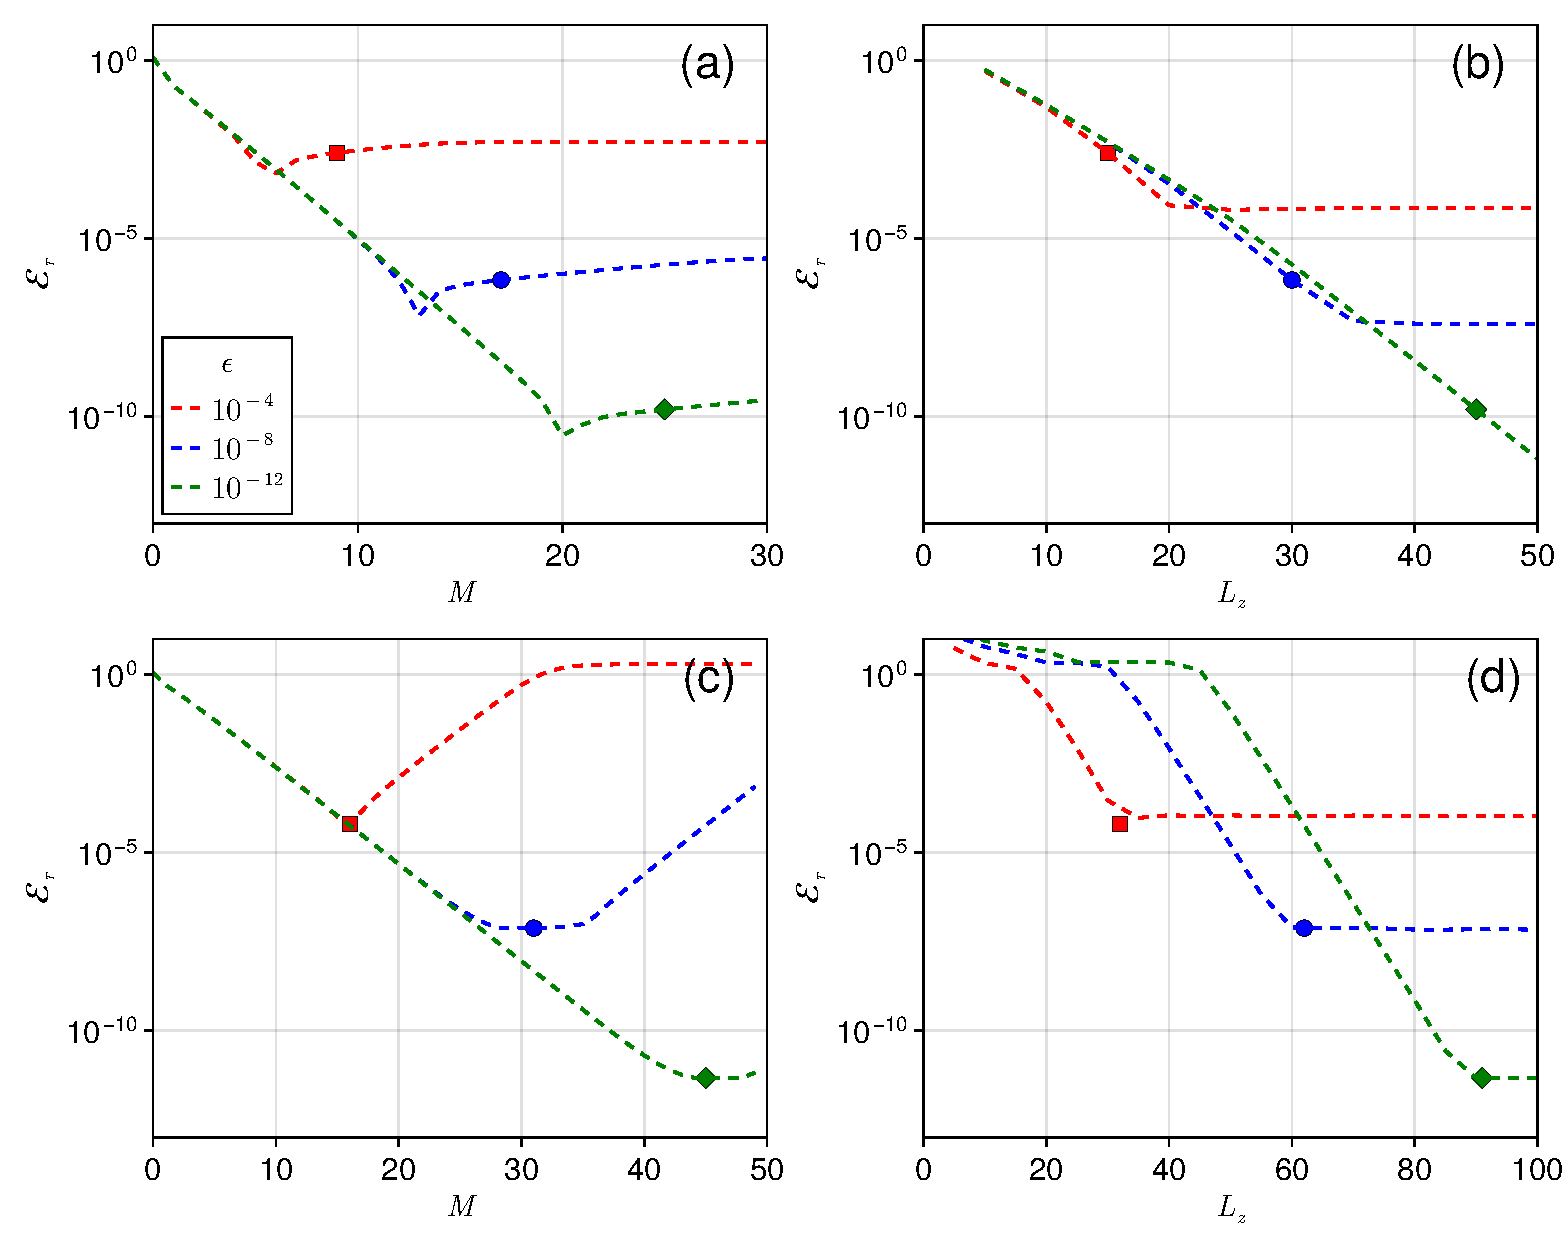
\includegraphics[width=0.92\linewidth]{figs/error_parameter_selection_force.pdf}
    \caption{
        Relative errors in force ($\mathcal{E}_r$) for two prototypical dielectric-confined systems with $\gamma=0.6$ (panels (a-b)) and $\gamma = 1$ (panels (c-d)), respectively.
        For both systems, we fix $L_x=L_y=10$ and $H = 1$. 
        Within each panel, the dashed lines correspond to the numerical errors obtained according to tolerance values $\epsilon = 10^{-4}$, $10^{-8}$, and $10^{-12}$, and the solid markers indicate the specific choice of $M$ or $L_z$ selected via the proposed strategy.
        Note that in panels (a) and (c), $s$ and $L_z$ are fixed according to Fig.~\ref{tab:parameter_selection_results}, whereas in panels (b) and (d), we fix $s$ and $M$.
    }
    \label{fig:error_parameter_selection_force}
\end{figure}
It is evident from Fig.~\ref{fig:error_parameter_selection_force} that, across all test cases with varying $\gamma$ and $\varepsilon$, the selected parameters consistently achieve optimal or near-optimal performance, especially for the case $\gamma = 1$. 
Consequently, we conclude that the parameter selection strategy proposed herein offers practical guidance for optimizing the performance of MD simulations of dielectric-confined systems.